\documentclass[10pt,a4paper]{article}
\usepackage[a4paper,margin=21mm]{geometry}
\usepackage[T1]{fontenc}
\usepackage{amsmath,txfonts,graphicx,booktabs,caption}
\usepackage[authoryear,round]{natbib}
\usepackage[hidelinks]{hyperref}
\captionsetup{font=small,labelfont=bf,skip=4pt,hypcap=false}
\setlength{\parindent}{0pt}
\setlength{\parskip}{4pt plus 1pt}
\setlength{\bibsep}{1pt}
\raggedbottom
\hypersetup{pdfauthor={Biswajit Jana},pdftitle={H-alpha measurements and optical aperture sizes in Euclid Deep Field North}}
\begin{document}
{\LARGE\bfseries H$\alpha$ measurements and optical aperture sizes\\[2pt] in Euclid Deep Field North\par}
\vspace{5pt}
{\large Biswajit Jana}\hfill 15 November 2026

\textbf{Abstract.} We use Euclid DR1-Foundation images and spectra to examine the association between measured H$\alpha$ flux and optical aperture radius in a $0.28^{\circ}$ field. Among 782 imaging-quality sources, the catalogue Kron-radius contrast between higher- and lower-flux emitters was $+0.05166$ dex. A comparison within tiles using direct VIS radii and reliable red-grism fluxes gave $+0.01402$ dex for 398 sources, with bootstrap endpoints of $-0.0173$ and $+0.0443$ dex. Of 356 sources with full nominal H$\alpha$ windows in both NISP grisms, none admitted strict fits in both. Including pixels flagged for low S/N yielded 14 dual detections at adjusted S/N $\geq 5$. Five remained above threshold after removal of the strongest red-core bin. These tests identify how imaging and spectral quality affect the measured contrast and isolate specific sources for further validation.

\section{Field and aperture measurements}
The pilot field is centred at ICRS RA $269.733^{\circ}$, Dec $+66.018^{\circ}$ \citep{aussel2026}. It contains 1576 exact catalogue matches across eight MER tiles, selected at $0.90\leq z\leq1.50$ with redshift probability $\geq0.99$, positive VIS aperture flux and a positive rank-0 H$\alpha$ fit at S/N $\geq5$. Imaging cuts require a positive Kron radius, zero VIS and detection flags, and spurious probability below 0.5. The smaller $0.15^{\circ}$ pilot matched morphology for 327 of 426 objects. It retained 150 after the same cuts, below its predeclared minimum of 200.

\begin{minipage}{\linewidth}
\centering
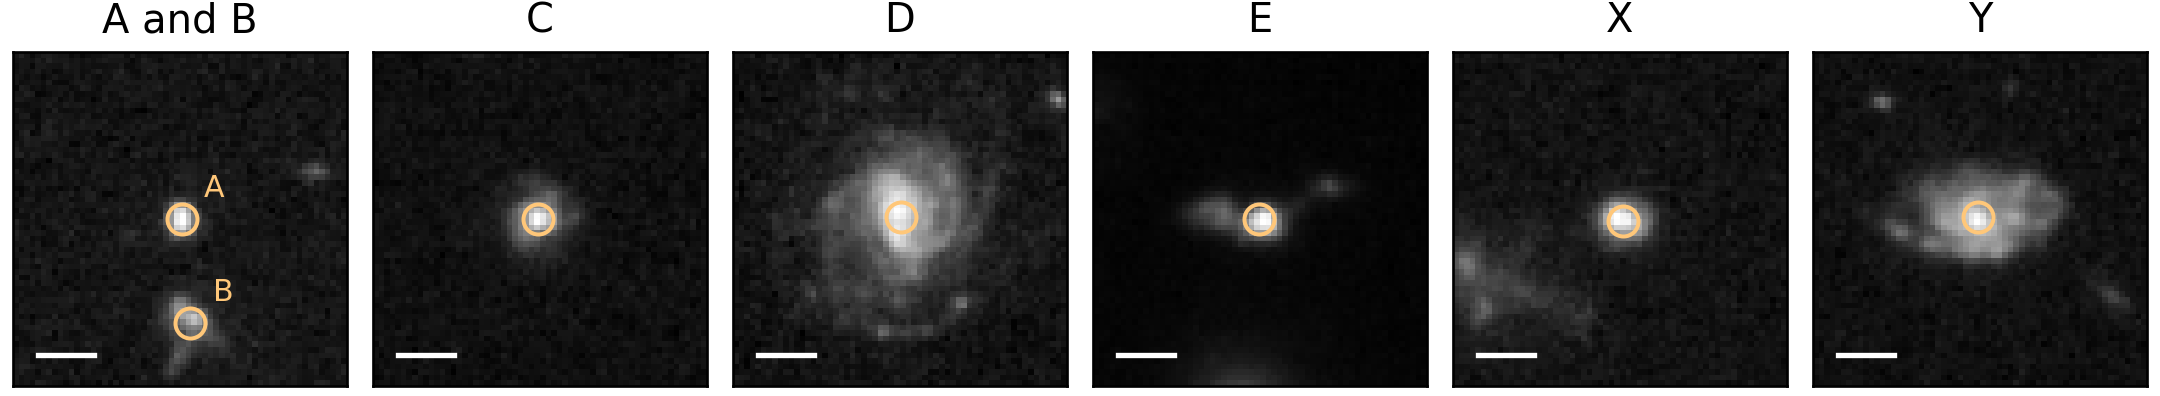
\includegraphics[width=\linewidth]{../analysis/euclid_vis_targets.png}
\captionof{figure}{Released Euclid MER VIS images of the seven objects discussed here. Circles mark their catalogue positions. The scale bar in each stamp is $1''$. The surface-brightness stretch is set separately for each panel.}
\label{fig:targets}
\end{minipage}

For each eligible cell, we subtract the median $\log_{10}r$ of the lower H$\alpha$ flux half from that of the upper half and average the differences weighted by cell population. Cells use redshift and VIS-flux strata. The direct radii enclose half the signed sky-subtracted VIS flux within $1.5''$. Their cells are also defined within tiles, with at least five objects per flux half. The direct analysis uses a $2.0''$ neighbour exclusion and 4000 whole-tile bootstrap draws. Five tiles supply eligible cells. Reliable red fluxes use SPE fit code 212.

\begin{minipage}{\linewidth}
\centering
\captionof{table}{Aperture-radius contrasts in the eight-tile field. The VIS rows use the same 398 galaxies. Intervals are descriptive bootstrap percentiles.}
\label{tab:radii}
\small
\begin{tabular}{@{}lrrrl@{}}
\toprule
Radius and line-flux measurement & $N$ & Contrast (dex) & 95\% endpoints (dex) & Resampling unit \\
\midrule
MER Kron, median catalogue H$\alpha$ & 782 & $+0.05166$ & $+0.0204$, $+0.0761$ & Objects \\
Direct VIS, median catalogue H$\alpha$ & 398 & $+0.03363$ & $-0.0116$, $+0.0710$ & Tiles \\
Direct VIS, reliable red-grism H$\alpha$ & 398 & $+0.01402$ & $-0.0173$, $+0.0443$ & Tiles \\
\bottomrule
\end{tabular}
\end{minipage}

Changing only the flux estimate in the direct comparison reduced the contrast by 0.01961 dex. At $2.5''$ isolation it was $+0.01719$ dex for 233 objects, with endpoints $-0.0211$ and $+0.0624$ dex. These aperture radii depend on the PSF and source profiles. The released sample is conditioned on line flux, so the pilot does not establish an intrinsic size relation.

\section{Spectral measurements}
Of 858 exact blue/red SIR matches in three archive partitions, 356 have a full $\pm250$~\AA{} nominal window in both grisms. We fit a local linear continuum and a $\sigma=30$~\AA{} Gaussian at the SPE-predicted H$\alpha$ wavelength. Fits require at least five usable core bins, at least 60\% coverage within $\pm45$~\AA, points on both sides of the centre, and five bins in each continuum sideband. Usable bins have quality $>0.8$ and mask 0 in the strict test. The alternate test also admits mask 2. The formal S/N is reduced when the sideband scatter exceeds the reported per-bin noise. The template can include [N~II] and its uncertainty excludes spectral covariance \citep{fumana2026,gabarra2026}.

\newpage
\section{Spectral results}
Strict fits are usable for 104 blue spectra and zero red spectra. Admitting mask 2 gives 22 dual fits and 14 with adjusted S/N $\geq5$ in both grisms. The same rules applied at offsets of $\pm300$ and $\pm440$~\AA{} give zero dual detections at that threshold in 87 usable windows. Of the 22 sources with usable centred fits, only one has usable fits at all five centres. The offset windows therefore provide a diagnostic, with insufficient matched coverage to calibrate a false-positive probability.

\begin{minipage}{\linewidth}
\centering
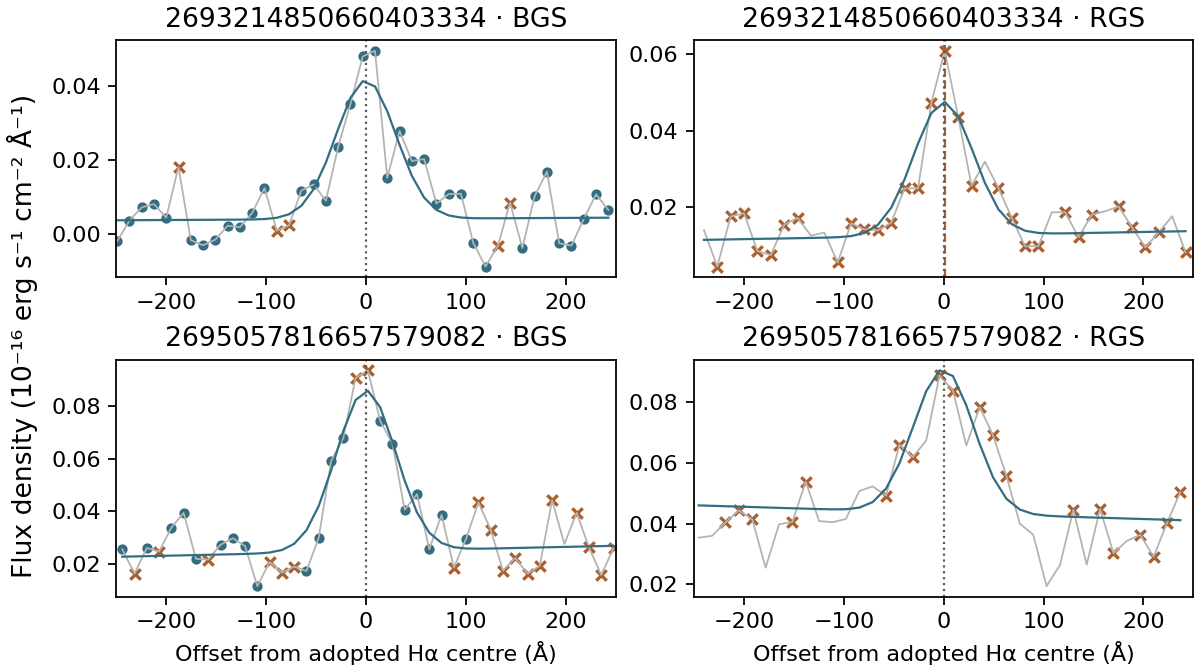
\includegraphics[width=.74\linewidth]{../../day03-cross-grism/analysis/example_spectra.png}
\captionof{figure}{Blue and red NISP windows for X (top, SPE-predicted centre) and Y (bottom, independent DESI centre). Crosses mark usable warning-flagged bins. The dashed line shows the red bin removed in the sensitivity check for X.}
\label{fig:spectra}
\end{minipage}

For X (MER 2693214850660403334), the blue and red adjusted S/N are 10.31 and 12.24. Removing the strongest red excess bin lowers red S/N to 9.17. Across all 14 candidates, five remain above threshold, one drops below it, and eight lose adequate fit coverage. Two candidates give dual detections at their independent DESI redshifts \citep{desi2025}. Y (MER 2695057816657579082) gives 13.29 and 9.23 at $z=0.905244$. Both DESI cases lose red coverage in the separate SPE-centred bin-removal check.

Fig.~\ref{fig:targets} also shows five comparison objects. A and B are distinct in Q1 and Subaru HSC imaging and lie $1.868''$ apart on the sky. A has strong H$\alpha$-region and [O~III] fits. B's H$\alpha$ fit depends on six warning-flagged core bins, leaving its redshift and any association with A uncertain. C has positive H$\alpha$-region flux in all 12 usable individual red extractions. D's combined formal S/N drops from 21.23 to 1.14 after one flagged bin is removed. E has strong blue H$\alpha$ and [O~III], and its DESI redshift of 0.975547 agrees with the Euclid value of 0.975754.

\textbf{Interpretation.} In 311 of 356 nominally overlapping sources, the red line core contains no strictly usable bins. The warning-inclusive candidates merit checks of individual exposures and contamination traces. No new source or redshift is established.

\textbf{Data and code.} The \href{https://github.com/Biswajit1999/daily-astro-notebooks/tree/master/euclid-dr1-foundation/edf-north-halpha}{study directory} contains source IDs, FITS cutouts, individual tests and reproduction commands. Euclid observations were obtained through NASA/IPAC IRSA. External observations are from Subaru HSC and DESI DR1.
\bibliographystyle{plainnat}
\bibliography{references}
\end{document}
